% ch12b Superconductivity in metals, part b (书页 205-232 / 分册p017-044)
\section{费米液体理论}

当然，我们的问题在某种程度上是人为的，因为我们忽略了除恰在费米面上方的那一对电子以外的所有电子间相互作用。一旦考虑全体电子之间的排斥相互作用，库珀失稳的简单图像理应失效，这是完全合理的预期。也就是说，当电子彼此相互作用时，我们不能先验地把无相互作用的本征态当作系统的有效描述（正如我们在库珀问题中所做的那样）。于是我们面临这样的问题：这种失稳是真实的吗？我们将从两条途径回答这一问题：一是借助费米面附近电子散射的简单物理考虑，二是借助对完整相互作用拉格朗日量作标度分析的更形式化的论证。如今人们普遍接受：金属的正常态由朗道–费米液体理论描述。按照这一理论，电子间相互作用在金属中的主导效应是重正化电子的有效质量，观测到的移动约为 10\% 到 50\% 的量级。费米液体理论的另一条本质论断是：金属正常态的激发态与无相互作用电子气的激发态之间存在一一对应。费米液体理论中的元激发称为准粒子（quasi-particle）。准粒子是一种具有寿命的复合粒子，其寿命源于与其他准粒子的碰撞。当准粒子的寿命 $\tau$ 为无穷大时，含这种粒子的态就是系统的本征态。然而，准粒子态要成为系统的本征态所必须满足的最低约束是 $\hbar/\tau\ll\tilde{\epsilon}_{\mathbf p}$，其中 $\tilde{\epsilon}_{\mathbf p}$ 是准粒子的能量。我们将在下文看到，当准粒子的能量趋近费米能级时，其寿命趋于无穷。准粒子在费米能级处的稳定性是费米液体理论的一条关键信条。

费米能级附近电子散射率趋于零可以证明如下。考虑一个接近 $T=0$ 的分布，其中除一个电子外所有电子都处于费米面以下。设 $\epsilon_1$ 为费米面之上那个电子的能量。具有该能量的电子要散射，必须与某个能量为 $\epsilon_2<\epsilon_{\mathrm F}$ 的电子相互作用。泡利不相容原理要求散射事件之后两个电子必须占据费米面以上的两个态。设这两个态的能量为 $\epsilon_3$ 与 $\epsilon_4$。能量守恒要求 $\epsilon_1+\epsilon_2=\epsilon_3+\epsilon_4$。若 $\epsilon_1=\epsilon_{\mathrm F}$，则为满足能量守恒，其余所有态也必须处于费米能级。因此，对处于费米能级的电子，可被散射进去的态数为零。于是，正比于散射态密度的散射率必定为零。结果是费米能级处电子或准粒子的寿命为无穷大。

\begin{figure}[H]\centering
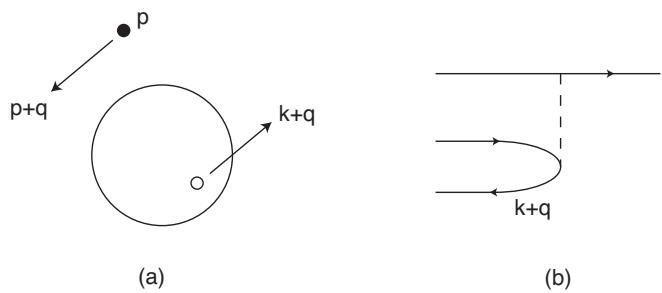
\includegraphics[width=0.62\textwidth]{figs/ch12/fig_12.12.jpg}
\caption*{图 12.12\quad（a）一个受激准粒子与基态中粒子的散射。（b）动量空间散射的图示表示。}\label{fig:auto:12.12}
\end{figure}

当 $\epsilon_1$ 离开费米能级时，存在一个宽度为 $\epsilon_1-\epsilon_{\mathrm F}$ 的态窗口，其余三个电子态可以从中选取。一旦从这个宽为 $\epsilon_1-\epsilon_{\mathrm F}$ 的窄窗中选定了其中两个态，由于能量守恒，最后一个态的能量便不能自由选取。因此，$\epsilon_2$ 有 $\epsilon_1-\epsilon_{\mathrm F}$ 种选择，$\epsilon_3$ 有 $\epsilon_1-\epsilon_{\mathrm F}$ 种选择，而 $\epsilon_4$ 随之确定。结果，散射率应当按 $(\epsilon_1-\epsilon_{\mathrm F})^2$ 标度。

为了更严格地看到这一点，我们计算动量态 $-\mathbf k$ 与 $-\mathbf k-\mathbf q$ 上的两个粒子散射到态 $\mathbf p$ 与 $\mathbf p+\mathbf q$ 的散射率。这一相互作用描绘于图 12.12。该过程的散射率为
\begin{equation*}
\frac{1}{\tau}=\frac{2\pi}{\hbar}\sum_{\mathbf q,\mathbf k,\sigma}|V(q)|^2 n_{\mathbf k\sigma}\left(1-n_{\mathbf k-\mathbf q\,\sigma}\right)\left(1-n_{\mathbf p+\mathbf q}\right)\delta\left(\hbar\omega_{\mathbf p\mathbf q}+\hbar\omega_{\mathbf k\mathbf q}\right), \tag{12.62}
\end{equation*}
其中 $V(q)$ 是库仑势的傅里叶变换，而 $\hbar\omega_{\mathbf p\mathbf q}=\epsilon_{\mathbf p+\mathbf q}-\epsilon_{\mathbf p}$。由能量守恒可得 $|\mathbf p+\mathbf q|<p$ 且 $|\mathbf p+\mathbf q|>p_{\mathrm F}$。这些条件概括为约束 $p_{\mathrm F}^2<|\mathbf p+\mathbf q|^2<p^2$，或者等价地
\begin{equation*}
p_{\mathrm F}^2-p^2<2pq\cos\theta+q^2<0. \tag{12.63}
\end{equation*}
正如我们在分析屏蔽时那样，可以利用自由粒子屏蔽函数的定义（见式 (9.103)）来简化对 $\mathbf k$ 的求和。在 $T=0$ 下，我们得到
\begin{equation*}
\frac{1}{\tau}=\frac{n_e}{2\hbar^2}\sum_{\mathbf q}|V(q)|^2 S_0(q,\hbar\omega_{\mathbf p\mathbf q})\left(1-n_{\mathbf p+\mathbf q}\right). \tag{12.64}
\end{equation*}
因为我们主要关注 $p-p_{\mathrm F}\approx 0$，故可取 $q$ 为小量。于是我们在托马斯–费米近似下取屏蔽库仑势的 $q\to 0$ 极限，$V(q\to 0)=4\pi e^2/V\kappa_{\mathrm{TF}}^2$。同时，取第 9 章导出的结构函数的 $q\to 0$ 形式：
\begin{equation*}
S(q,\omega_{\mathbf p\mathbf q})\propto\frac{\omega_{\mathbf p\mathbf q}}{q}. \tag{12.65}
\end{equation*}
因此，散射率简化为
\begin{equation*}
\frac{1}{\tau}\propto\frac{1}{\epsilon_{\mathrm F}}\int\sin\theta\,\mathrm d\theta\int q\,\omega_{\mathbf p\mathbf q}\,\mathrm d q. \tag{12.66}
\end{equation*}
通过求解 $\hbar\omega_{\mathbf p\mathbf q}=(2pq\cos\theta+q^2)/2m$，我们可以把对 $q$ 的积分换成对 $\omega_{\mathbf p\mathbf q}$ 的积分。散射率正比于
\begin{align*}
\frac{1}{\tau}&\propto\frac{1}{\epsilon_{\mathrm F}}\int_0^{\epsilon_{\mathrm p}-\epsilon_{\mathrm F}}\mathrm d\omega\int_{-1}^{1}\omega\left(1-\frac{xp_{\mathrm F}}{\sqrt{x^2p_{\mathrm F}^2+\omega}}\right)\mathrm d x\\
&\propto\frac{1}{\epsilon_{\mathrm F}}\int_0^{\epsilon_{\mathrm p}-\epsilon_{\mathrm F}}\omega\,\mathrm d\omega\propto\frac{(\epsilon_{\mathrm p}-\epsilon_{\mathrm F})^2}{\epsilon_{\mathrm F}}. \tag{12.67}
\end{align*}
于是我们清楚地看到，散射率按 $(\epsilon_{\mathbf p}-\epsilon_{\mathrm F})^2$ 标度，因而在费米能级处的态上为零。取 $\epsilon_{\mathbf p}-\epsilon_{\mathrm F}\propto k_{\mathrm B}T$，我们发现散射率正比于 $T^2$。正如上一章所述，铜氧化物高温 $T_{\mathrm c}$ 材料正常态的电阻率 [GF1987] 在直到 $T_{\mathrm c}$ 的温区内随温度线性变化。对照费米液体的结果，这种行为强烈暗示这些材料的正常态是非费米液体。

准粒子散射率对温度的二次依赖是费米液体理论的一个核心预言。室温下 $(k_{\mathrm B}T)^2/\epsilon_{\mathrm F}$ 的量级为 $10^{-4}\,\mathrm{eV}$。由此给出的散射寿命在室温下为 $10^{-10}\,\mathrm{s}$ 的量级。金属中典型的弛豫时间比这短四个数量级（见第 11 章）。因此，电子–电子相互作用并不是费米能级附近电子的主导散射机制。正因如此，无相互作用的图像才如此有效，是金属正常态性质的良好近似——至少在室温下如此。当然，在足够低的温度下，电子–电子相互作用的重要性急剧增大，超导电性就是一个现成的例子。

费米液体理论的终极表述 [P1992; SM1991; BG1990] 是：短程排斥相互作用在费米面处是无关的（irrelevant）。一旦我们建立起关于费米子相干态的若干预备结果，这一表述便可以从相互作用系统的拉格朗日量的标度分析中得到证明。费米子相干态与费米子算符 $\Psi$ 由本征值方程
\begin{equation*}
\Psi|\psi\rangle=\psi|\psi\rangle, \tag{12.68}
\end{equation*}
相联系，其中 $|\psi\rangle$ 是费米子相干态。然而，本征值 $\psi$ 并非普通的数。它的平方 $\psi^2$ 为零，从而蕴含如下一系列等式
\begin{equation*}
\Psi^2|\psi\rangle=\psi^2|\psi\rangle=0|\psi\rangle \tag{12.69}
\end{equation*}
成立。$\psi$ 是一个格拉斯曼（Grassmann）变量，即一个反对易的数。虽然这看似古怪，但格拉斯曼数的平方为零恰恰是我们在费米子路径积分表述中把泡利原理纳入其中的所需之物。

那么，使式 (12.68) 成为可能的态 $|\psi\rangle$ 究竟是什么？我们作如下拟设（ansatz）
\begin{equation*}
|\psi\rangle=|0\rangle-\psi|1\rangle \tag{12.70}
\end{equation*}
它符合费米子相干态的要求。这里 $\Psi|0\rangle=0=\Psi^\dagger|1\rangle=0$ 且 $\Psi|1\rangle=|0\rangle$。我们按如下方式检验该拟设，首先注意
\begin{equation*}
\Psi|\psi\rangle=-\Psi\psi|1\rangle=\psi\Psi|1\rangle=\psi|0\rangle. \tag{12.71}
\end{equation*}
然而 $|0\rangle=|\psi\rangle+\psi|1\rangle$。代入后得到
\begin{equation*}
\Psi|\psi\rangle=\Psi\left[|\psi\rangle+\psi|1\rangle\right]=\psi|\psi\rangle, \tag{12.72}
\end{equation*}
此即所求。因此 $|\psi\rangle$ 构成一个费米子相干态。现在考虑伴随 $\langle\bar\psi|\Psi^\dagger$。量子力学的标准规则可以应用于伴随。例如
\begin{equation*}
\langle\bar\psi|\Psi^\dagger\equiv\langle\bar\psi|\bar\psi. \tag{12.73}
\end{equation*}
利用 $\bar\psi\langle 1|=-\langle 1|\bar\psi$ 这一事实，我们得到
\begin{align*}
\langle\bar\psi|\psi\rangle&=\langle 0|0\rangle+\bar\psi\psi\langle 1|1\rangle\\
&=1+\bar\psi\psi=\mathrm e^{\bar\psi\psi}. \tag{12.74}
\end{align*}
这个表达式可能显得有些奇怪，因为截断绝非源于 $\bar\psi\psi$ 的小。这个量既不大也不小。截断之所以成立，是因为格拉斯曼变量的平方为零。

继续往下，我们需要几个积分：
\begin{equation*}
\int\psi\,\mathrm d\psi=1, \tag{12.75}
\end{equation*}
\begin{equation*}
\int\mathrm d\psi=\int\mathrm d\bar\psi=0, \tag{12.76}
\end{equation*}
\begin{equation*}
\int\bar\psi\psi\,\mathrm d\bar\psi\,\mathrm d\psi=-1, \tag{12.77}
\end{equation*}
\begin{equation*}
\int\mathrm e^{-a\bar\psi\psi}\mathrm d\bar\psi\,\mathrm d\psi=\int\left(1-a\bar\psi\psi\right)\mathrm d\bar\psi\,\mathrm d\psi=a, \tag{12.78}
\end{equation*}
\begin{equation*}
\int\mathrm e^{-\bar\psi M\psi}\mathrm d\bar\psi\,\mathrm d\psi=\mathrm{Det}\,M. \tag{12.79}
\end{equation*}
这些积分使我们能够建立若干恒等式。首先是恒等算符的分解，
\begin{equation*}
\int|\psi\rangle\langle\bar\psi|\mathrm e^{-\bar\psi\psi}\mathrm d\bar\psi\,\mathrm d\psi=|0\rangle\langle 0|+|1\rangle\langle 1|=I, \tag{12.80}
\end{equation*}
它在费米子相干态的表述下具有格外简单的形式。在用费米子相干态写出路径积分时，我们还需要玻色型算符的迹的表达式。所谓玻色型，我们只是指由偶数个费米子算符构成的算符。考虑量
\begin{align*}
\langle-\bar\psi|\psi\rangle&=\left[\langle 0|-\bar\psi\langle 1|\right]\left[|0\rangle-\psi|1\rangle\right]\\
&=\langle 0|0\rangle-\bar\psi\psi\langle 1|1\rangle. \tag{12.81}
\end{align*}
为得到对角元之和，我们计算积分
\begin{equation*}
\int\left[\langle 0|0\rangle-\bar\psi\psi\langle 1|1\rangle\right]\mathrm e^{-\bar\psi\psi}\mathrm d\bar\psi\,\mathrm d\psi=\langle 0|0\rangle+\langle 1|1\rangle. \tag{12.82}
\end{equation*}
因此，迹公式为
\begin{equation*}
\mathrm{Tr}\,\Omega=\int\langle-\bar\psi|\Omega|\psi\rangle\mathrm e^{-\bar\psi\psi}\mathrm d\bar\psi\,\mathrm d\psi. \tag{12.83}
\end{equation*}

利用这些关系，我们来表达配分函数
\begin{equation*}
Z=\mathrm{Tr}\,\mathrm e^{-\beta H}, \tag{12.84}
\end{equation*}
把它写成相干态的形式。通过与标准薛定谔传播子的类比，我们把 $\beta$ 确认为一个虚时间。我们用 $\epsilon=\beta/N$ 对这个“时间”区间作细分，并把玻尔兹曼权重
\begin{equation*}
Z=\lim_{N\to\infty}\mathrm{Tr}\left[\mathrm e^{-\epsilon H}\right]^N \tag{12.85}
\end{equation*}
提升到 $N$ 次幂。在大 $N$ 极限下，我们可以把指数因子截断到第一项。为紧凑起见，我们定义 $\hat D_\epsilon\equiv\hat D_\epsilon(\psi^\dagger,\psi)=1-\epsilon H$。然后利用谱分解的单位元，即式 (12.80)，得到
\begin{align*}
Z=\int{}&\langle-\bar\psi_0|\hat D_\epsilon|\psi_{N-1}\rangle\mathrm e^{-\bar\psi_{N-1}\psi_{N-1}}\langle\bar\psi_{N-1}|\hat D_\epsilon|\psi_{N-2}\rangle\mathrm e^{\bar\psi_{N-2}\psi_{N-2}}\\
&\times\langle\bar\psi_{N-2}|\cdots|\psi_1\rangle\mathrm e^{-\bar\psi_1\psi_1}\langle\bar\psi_1|\hat D_\epsilon|\psi_0\rangle\mathrm e^{-\bar\psi_0\psi_0}\prod_{i=0}^{N-1}\mathrm d\bar\psi_i\,\mathrm d\psi_i \tag{12.86}
\end{align*}
作为配分函数的工作表达式。假定 $H$ 中所有算符都是正规序的，使得 $H|0\rangle=0$。于是
\begin{equation*}
\langle\bar\psi_{i+1}|\hat D_\epsilon|\psi_i\rangle=\langle\bar\psi_{i+1}|D_\epsilon(\psi^\dagger_{i+1},\psi_i)|\psi_i\rangle=\mathrm e^{\bar\psi_{i+1}\psi_i}\mathrm e^{-\epsilon H(\psi^\dagger_{i+1},\psi_i)}. \tag{12.87}
\end{equation*}
大功告成在即。我们只需把式 (12.87) 代入式 (12.86) 共 $N$ 次，
\begin{equation*}
Z=\lim_{N\to\infty}\int\prod_{i=0}^{N-1}\mathrm e^{\left[\left(\frac{(\bar\psi_{i+1}-\bar\psi_i)}{\epsilon}\psi_i-H\right)\epsilon\right]}\mathrm d\bar\psi_i\,\mathrm d\psi_i, \tag{12.88}
\end{equation*}
其中我们定义了 $\bar\psi_N=-\bar\psi_0$ 与 $\psi_N=-\psi_0$，且 $\psi_N$ 与 $\bar\psi_N$ 明确不参与积分。在 $N\to\infty$ 极限下，可以把指数中的求和化为积分。对时间导数项分部积分并利用边界条件 $\psi(0)=\psi(\beta)=0$，我们把配分函数化为标准形式
\begin{equation*}
Z=\int\mathcal D\bar\psi\,\mathcal D\psi\,\mathrm e^{-S_{\mathrm E}}, \tag{12.89}
\end{equation*}
其中 $S_{\mathrm E}$
\begin{equation*}
S_{\mathrm E}=\int\left(\bar\psi\partial_\tau\psi+H\right)\mathrm d^d x\,\mathrm d\tau, \tag{12.90}
\end{equation*}
是欧几里得作用量，$\tau$ 的积分在区间 $[0,\beta]$ 上进行。这是一切费米子量子场论的出发点。

考虑无相互作用电子的情形。哈密顿量
\begin{equation*}
H=\sum_{\mathbf p,\sigma}\left(\epsilon_{\mathbf p}-\epsilon_{\mathrm F}\right)\psi^\dagger_\sigma(\mathbf p)\psi_\sigma(\mathbf p), \tag{12.91}
\end{equation*}
用动量空间的产生与湮灭算符写出十分方便，其中 $\epsilon(\mathbf p)$ 是自由粒子色散关系，$\epsilon_{\mathrm F}$ 是费米能。相应的作用量为
\begin{equation*}
S=\int\mathrm d t\,\mathrm d^3\mathbf p\left(\mathrm i\psi^\dagger_\sigma(\mathbf p)\partial_t\psi_\sigma(\mathbf p)-\psi^\dagger_\sigma(\mathbf p)\left(\epsilon_{\mathbf p}-\epsilon_{\mathrm F}\right)\psi_\sigma(\mathbf p)\right), \tag{12.92}
\end{equation*}
这里我们已经换到实时间。严格说来，作用量应当用费米子相干态而不是费米子产生、湮灭算符来写。虽然这一区别对我们这里考虑的应用并不关键，但在费米子路径积分中使用费米子相干态却是至关重要的。尽管如此，约定俗成的是：用产生、湮灭算符写出的路径积分实际上暗含以相干态为工作基。

我们希望考虑朝向费米面的标度变换。首先需要引入标度维数的概念。考虑简单函数 $f(x)=x^2$。在标度 $x\to sx$ 下，$f(x)\to s^2x^2$，其中假定 $s$ 为正。若 $s\to 0$，函数 $f$ 随之消失。我们把参数 $x$ 的标度维数定义为：为得到 $x$ 的标度变换，标度因子 $s$ 必须被提升到的幂次。操作上，
\begin{equation*}
\mathrm{Dim}[x]=\frac{\mathrm d f}{\mathrm d s}\frac{s}{f}=\frac{\mathrm d\ln f}{\mathrm d\ln s}=2. \tag{12.93}
\end{equation*}
在场论的语境下，标度维数起着基本作用。让我们把作用量分割为
\begin{equation*}
S=S_0+S_{\mathrm{int}}, \tag{12.94}
\end{equation*}
其中所有相互作用都包含在
\begin{equation*}
S_{\mathrm{int}}=\int\mathrm d t\,\mathrm d^d\mathbf k\,\mathcal O(\mathbf k,t) \tag{12.95}
\end{equation*}
之中。这里 $\mathcal O$ 是某个算符（当然是由基本场构成的复合算符），它决定相互作用。我们这样选取时间、动量和裸场的标度，使得 $S_0\to s^0S_0=S_0$。在这种标度选取下，相互作用项将变换为 $s^bS_{\mathrm{int}}$。若 $b>0$，则由 $\mathcal O$ 生成的相互作用是无关的，因为它们在标度极限下消失；此时我们称 $\mathcal O$ 为无关算符。若 $b<0$，则 $\mathcal O$ 是相关的。$b=0$ 时出现边际（marginal）情形。由于我们考虑的是朝向费米面的标度，我们希望这样标度所有的场与空间、时间坐标，使相关的自由粒子作用量的标度维数为零。随后我们将证明：把同样的标度用于任何排斥性短程四费米子相互作用时，只要 $d\ge 2$，其标度维数必为正。跟随波尔钦斯基（Polchinski）[P1992]，我们把一个电子的动量写作
\begin{equation*}
\mathbf p=\mathbf k+\boldsymbol\ell, \tag{12.96}
\end{equation*}
即两个动量之和：一个位于费米面上（$\mathbf k$），另一个垂直于它（$\boldsymbol\ell$），后者代表对费米面的偏离。于是，我们在费米面附近展开电子的色散关系
\begin{equation*}
\epsilon(\mathbf p)=\epsilon_{\mathrm F}+\ell\frac{\partial\epsilon}{\partial\mathbf p}+O(\ell^2), \tag{12.97}
\end{equation*}
只保留线性项。由于能量零点取在费米面上，保持费米面不变的相关标度变换为 $\mathbf k\to\mathbf k$、$\ell\to s\ell$ 以及 $E\to sE$。作为能量这一标度的结果，
\begin{equation*}
\frac{\partial}{\partial t}\to s\frac{\partial}{\partial t}, \tag{12.98}
\end{equation*}
这意味着 $t\to s^{-1}t$。类似地，$\mathrm d^d\mathbf p\to\mathrm d^{d-1}\mathbf k\,\mathrm d(s\ell)$。在这些标度变换下，作用量
\begin{equation*}
s\int\mathrm d t\,\mathrm d^{d-1}\mathbf k\,\mathrm d\ell\left(\mathrm i\psi^\dagger_\sigma(\mathbf p)\partial_t\psi_\sigma(\mathbf p)-\ell v_{\mathrm F}\psi^\dagger_\sigma(\mathbf p)\psi_\sigma(\mathbf p)\right), \tag{12.99}
\end{equation*}
以 $s$ 线性标度，再乘以乘积 $\psi^\dagger_\sigma(\mathbf p)\psi_\sigma(\mathbf p)$ 的标度维数。要使作用量的标度维数为零，我们必须如下标度场：
\begin{equation*}
\psi_\sigma(\mathbf p)\to s^{-1/2}\psi_\sigma(\mathbf p), \tag{12.100}
\end{equation*}
以吸收来自 $\ell$ 与能量标度的整体 $s$ 因子。由标度维数的定义可得
\begin{equation*}
\mathrm{Dim}\left[\psi_\sigma(\mathbf p)\right]=-\frac{1}{2}. \tag{12.101}
\end{equation*}
于是我们费米面上的理论具有零标度维数。然而，我们还没有指明化学势。这样一个项
\begin{equation*}
\int\mathrm d t\,\mathrm d^{d-1}\mathbf k\,\mathrm d\ell\,\mu(\mathbf k)\psi^\dagger_\sigma(\mathbf p)\psi_\sigma(\mathbf p), \tag{12.102}
\end{equation*}
在我们的有效低能理论中取质量项的形式。该项按 $s^{-1+1-2/2}=s^{-1}$ 标度。因此这一项总是相关的。尽管如此，它可以被吸收进动能项，这意味着我们围绕费米面展开的参照是完全填满的态，而不是一个（方便地）可视为空置的真空。

如果不存在相关微扰，理论就是自然的。考虑短程四费米子相互作用项
\begin{equation*}
\int\mathrm d t\prod_{i=1}^{4}\mathrm d^{d-1}\mathbf k_i\,\mathrm d\ell_i\,V(\mathbf k_1,\ldots,\mathbf k_4)\psi^\dagger_\sigma(\mathbf p_1)\psi_\sigma(\mathbf p_3)\psi^\dagger_{\sigma'}(\mathbf p_2)\psi_{\sigma'}(\mathbf p_4)\delta^d(\mathbf p_1+\mathbf p_2-\mathbf p_3-\mathbf p_4). \tag{12.103}
\end{equation*}
此处 $V$ 的符号还是任意的。我们聚焦于短程相互作用是有根据的，因为我们已经证明，在金属密度下金属中的相互作用被良好屏蔽。在自由部分作用量所用的标度下，我们发现相互作用项按 $s^{4-1-4/2}=s$ 标度，再乘以 $\delta$ 函数的标度。$s^4$ 因子来自四个 $\mathrm d\ell$ 因子，$s^{-1}$ 来自时间积分，$s^{-2}$ 来自四个场因子 $\psi_\sigma(\mathbf p)$。那么 $\delta$ 函数的标度如何？如果简单地把式 (12.96) 代入 $\delta$ 函数的自变量，我们发现
\begin{align*}
\delta^d(\mathbf p_1+\mathbf p_2-\mathbf p_3-\mathbf p_4)&=\delta^d(\mathbf k_1+\mathbf k_2-\mathbf k_3-\mathbf k_4+\mathrm l_1+\mathrm l_2-\mathrm l_3-\mathrm l_4)\\
&\approx\delta^d(\mathbf k_1+\mathbf k_2-\mathbf k_3-\mathbf k_4). \tag{12.104}
\end{align*}
因此 $\delta$ 函数不参与标度，我们得出结论：短程相互作用在费米面上是无关的，因为它们随 $s$ 线性标度。

然而，这一论证对费米面让步太多。超导电性毕竟可以理解为费米面对吸引接触相互作用的不稳定性。因此上述论证过于宽泛。我们通过考虑由大动量连接的散射过程来微调这一论证，以此作为超导问题的先导——在超导问题中，散射发生在费米面两侧的电子之间，如图 12.13 所描绘。具体地，考虑动量为 $\mathbf p_1$ 与 $\mathbf p_2$ 的一对电子散射到动量为 $\mathbf p_3$ 与 $\mathbf p_4$ 的态。一开始，我们考虑 $\mathbf p_1$ 与 $\mathbf p_2$ 之间没有任何特殊关系的一般情形，如图 12.13 所示。我们把散射后的动量写作 $\mathbf p_3=\mathbf p_1+\delta\mathbf k_3+\delta\boldsymbol\ell_3$ 与 $\mathbf p_4=\mathbf p_2+\delta\mathbf k_4+\delta\boldsymbol\ell_4$。动量守恒条件此时变为
\begin{equation*}
\delta^d\left(\delta\mathbf k_3+\delta\mathbf k_4+\delta\boldsymbol\ell_3+\delta\boldsymbol\ell_4\right). \tag{12.105}
\end{equation*}

\begin{figure}[H]\centering
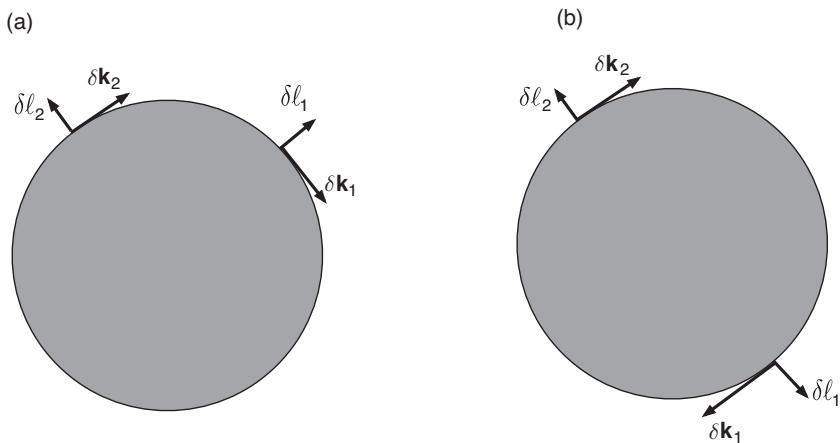
\includegraphics[width=0.62\textwidth]{figs/ch12/fig_12.13.jpg}
\caption*{图 12.13\quad（a）两个电子一般地位于费米面上的动量。（b）此处两动量相反，即 $\mathbf p_1=-\mathbf p_2$。这时 $\delta\mathbf k_1$ 与 $\delta\mathbf k_2$ 平行，且 $\delta\boldsymbol\ell_1$ 与 $\delta\boldsymbol\ell_2$ 指向恰好相反的方向。}\label{fig:auto:12.13}
\end{figure}

当诸 $\delta\mathbf k_i$ 线性无关时，$\delta$ 函数可以像之前那样处理。具体地说，它不参与标度，我们之前的结论——四费米子相互作用是无关的——依然成立。考虑图 12.13b 所示的情形，其中 $\mathbf p_1=-\mathbf p_2$，因而 $\delta\mathbf k_3$ 与 $\delta\mathbf k_4$ 彼此平行。此时，维持动量守恒的 $\delta$ 函数
\begin{equation*}
\delta^d\left(\delta\mathbf k_3+\delta\mathbf k_4\right)\delta^d\left(\delta\boldsymbol\ell_3+\delta\boldsymbol\ell_4\right), \tag{12.106}
\end{equation*}
发生因子化，因为 $\delta\boldsymbol\ell_3$ 与 $\delta\boldsymbol\ell_4$ 都垂直于 $\delta\mathbf k_3$ 与 $\delta\mathbf k_4$。在标度 $\ell\to s\ell$ 下，两个 $\delta$ 函数中的第二个按 $s^{-1}$ 标度。该因子抵消了先前导出的线性 $s$ 因子。因此我们相当普遍地发现：当这对电子的净动量为零时，四费米子相互作用既不相关也非无关，而是按 $s^0$ 标度，因而是边际的。

那么这把我们置于何地？当电子散射到宇称对称的动量态时，我们需要更加努力地弄清费米面的命运。为此，我们计算一阶修正，希望构造一个类似于近藤问题中交换耦合的递推关系。到 $V^2$ 阶，相关的图示于图 12.14。第一张图就是裸电子–电子相互作用顶点。第二张图是精确到相互作用二阶的顶点。我们赋予气泡（即图中的诸线）的每条内部费米子线一个形式为 $1/(E-v_{\mathrm F}\ell)$ 的传播子，其中 $E$ 是内部费米子线的能量。二阶顶点取如下形式
\begin{equation*}
V^2\int\frac{\mathrm d E'\,\mathrm d^2\mathbf k\,\mathrm d\ell'}{2\pi^4}\frac{1}{\left[(1+\mathrm i\epsilon)(E+E')-v_{\mathrm F}(\mathbf k')\ell'\right]\left[(1+\mathrm i\epsilon)(E-E')-v_{\mathrm F}(\mathbf k')\ell'\right]}. \tag{12.107}
\end{equation*}

\begin{figure}[H]\centering
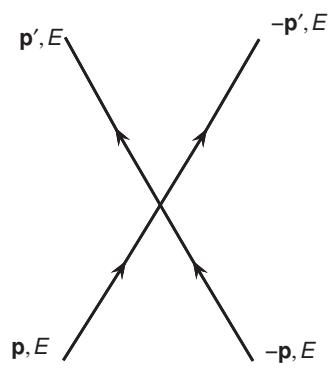
\includegraphics[width=0.40\textwidth]{figs/ch12/fig_12.14_a.jpg}\hfill
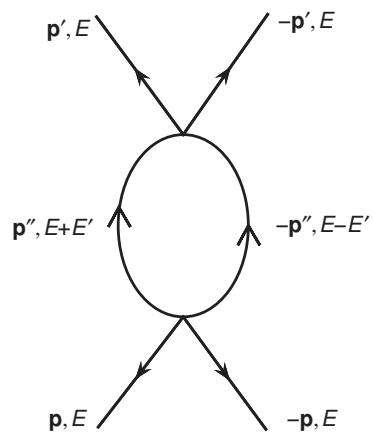
\includegraphics[width=0.40\textwidth]{figs/ch12/fig_12.14_b.jpg}
\caption*{图 12.14\quad（a）处于态 $(\mathbf p,E)$ 与 $(-\mathbf p,E)$ 的电子散射到 $(-\mathbf p',E)$ 与 $(-\mathbf p',E)$ 的裸相互作用顶点；（b）$O(V^2)$ 顶点。与该顶点对应的积分在式 (12.107) 中计算。}\label{fig:auto:12.14}
\end{figure}

$(1+\mathrm i\epsilon)$ 因子的作用是正规化积分。最后我们将取 $\epsilon\to 0$ 极限。在计算气泡顶点中的积分时，把分母改写为
\begin{equation*}
\frac{-1}{(1+2\mathrm i\epsilon)\left[E'+E-(1-\mathrm i\epsilon)v_{\mathrm F}(\mathbf k')\ell'\right]\left[E'-E+(1-\mathrm i\epsilon)v_{\mathrm F}(\mathbf k')\ell'\right]}, \tag{12.108}
\end{equation*}
会有所帮助，其中我们明确地做了近似 $(1+\mathrm i\epsilon)^2\approx(1+2\mathrm i\epsilon)$，因为 $\epsilon$ 严格属于 $O(0)$ 阶。为计算该积分，我们在上半平面闭合围道。有两个我们感兴趣的极点，位于
\begin{equation*}
E'=\pm E\mp v_{\mathrm F}(\mathbf k')\ell'\pm\mathrm i\epsilon v_{\mathrm F}(\mathbf k')\ell', \tag{12.109}
\end{equation*}
其中上号对应 $\ell'>0$，下号对应 $\ell'<0$，这样两个极点都位于上半平面。利用每个极点处的留数为
\begin{equation*}
\frac{2\pi\mathrm i}{\pm 2E\mp 2v_{\mathrm F}(\mathbf k')\ell'\pm 2\mathrm i\epsilon v_{\mathrm F}(\mathbf k')\ell'}, \tag{12.110}
\end{equation*}
这一事实，我们把二阶顶点化为
\begin{equation*}
\frac{-\mathrm i V^2}{2}N\left[\int_0^{E_0}\frac{\mathrm d b}{E-b+\mathrm i\epsilon}+\int_{-E_0}^{0}\frac{\mathrm d b}{b-E-\mathrm i\epsilon}\right], \tag{12.111}
\end{equation*}
其中已换元 $b=v_{\mathrm F}(\mathbf k')\ell'$，并定义了
\begin{equation*}
N=\int\frac{\mathrm d^2\mathbf k'}{(2\pi)^3}\frac{1}{v_{\mathrm F}(\mathbf k')}, \tag{12.112}
\end{equation*}
同时忽略了正比于无穷小量 $\epsilon$ 的各项之前的任何前置因子。每个积分都给出一个对数：
\begin{equation*}
\mathrm i V^2N\ln\left(\frac{E_0}{|E|}\right). \tag{12.113}
\end{equation*}
注意到裸四费米子顶点正比于 $-\mathrm i V$，精确到二阶的有效相互作用变为
\begin{equation*}
V(E)=V-V^2N\left(\ln\left(\frac{E_0}{|E|}\right)+O(1)\right)+O(V^3). \tag{12.114}
\end{equation*}
我们对这个等式的两边求导，
\begin{equation*}
\frac{\mathrm d V(E)}{\mathrm d E}=NV(E)^2/E, \tag{12.115}
\end{equation*}
得到相互作用顶点的标度方程。这个方程与第 8 章近藤问题中导出的交换相互作用增长的标度方程完全相同。该方程的解就是
\begin{equation*}
V(E)=\frac{V}{1+NV\ln(E_0/E)}. \tag{12.116}
\end{equation*}
我们清楚地看到：对于正的裸相互作用 $V>0$，有效相互作用在低能（即 $E<E_0$）处减小。然而，对 $V<0$，相互作用增大。这就是 BCS 失稳，也是如下的基本论断：除短程吸引外，所有重正化都朝向费米面。注意，裸相互作用 $V$ 是真正的边际量。因此，BCS 理论中的超导电性是边际耦合变大并在强耦合处产生新自由度（即电子对凝聚）的一个例子。

BCS 超导配对理论的一个关键假设是：正常态的性质由具有无穷寿命 [L1964; L1965] 的无相互作用准粒子描述，且这些准粒子与裸电子一一对应。这一假设得到刚才给出的标度分析的支持，也在从 I 类到 II 类的众多材料的正常态中得到实验支持。由于正常态本质上无相互作用，某个准粒子的能量就是把该粒子加入或移出系统某个态所需的能量。为说明这一概念，考虑一个由某分布函数 $n^0_{\mathbf p\sigma}$（一般取为费米–狄拉克分布）描述的相互作用系统。设想以极其缓慢的方式向系统加入或移出一个粒子，使系统始终处于基态。这一过程代表粒子数的绝热改变。尽管如此，这一过程会把粒子分布改变为某个新量 $n_{\mathbf p\sigma}$，从而基态能量也随之改变。设 $\delta n_{\mathbf p\sigma}$ 表示粒子分布函数的相应改变。我们可以把基态能量的变化
\begin{equation*}
\delta E=\frac{1}{V}\sum_{\mathbf p\sigma}\epsilon_{\mathbf p\sigma}\delta n_{\mathbf p\sigma}+\frac{1}{2V^2}\sum_{\mathbf p\sigma,\mathbf p'\sigma'}f_{\mathbf p\sigma,\mathbf p'\sigma'}\delta n_{\mathbf p\sigma}\delta n_{\mathbf p'\sigma'}+\cdots, \tag{12.117}
\end{equation*}
按涨落 $\delta n_{\mathbf p\sigma}$ 的幂次展开而计算出来。朗道 [L1956] 参量 $f_{\mathbf p\sigma,\mathbf p'\sigma'}$ 描述准粒子之间如何相互作用。该量在 $\mathbf p$ 与 $\mathbf p'$ 互换下不变。我们把准粒子的能量
\begin{equation*}
\tilde\epsilon_{\mathbf p\sigma}=\epsilon_{\mathbf p\sigma}+\frac{1}{V}\sum_{\mathbf p'\sigma'}f_{\mathbf p\sigma,\mathbf p'\sigma'}\delta n_{\mathbf p'\sigma'}+\cdots, \tag{12.118}
\end{equation*}
通过对新基态能量关于 $\delta n_{\mathbf p\sigma}$ 求变分而识别出来。于是我们清楚地看到，准粒子能量本身是分布函数的函数。更明确地说，准粒子服从费米–狄拉克分布函数，只是把 $\epsilon_{\mathbf p}-\mu$ 换成了 $\tilde\epsilon_{\mathbf p_\sigma}-\mu$。在费米面上，准粒子以下列速度运动：
\begin{equation*}
v_{\mathrm F}=\left(\frac{\partial\epsilon_{\mathbf p\sigma}}{\partial\mathbf p}\right)_{p=p_{\mathrm F}} \tag{12.119}
\end{equation*}
它等于费米速度。因为 $v_{\mathrm F}=p_{\mathrm F}/m^*$，准粒子有效质量的形式定义为
\begin{equation*}
\frac{1}{m^*}=\frac{1}{p_{\mathrm F}}\left(\frac{\partial\epsilon_{\mathbf p\sigma}}{\partial\mathbf p}\right)_{p=p_{\mathrm F}}. \tag{12.120}
\end{equation*}
因此在费米面附近，准粒子能量
\begin{equation*}
\epsilon_{\mathbf p\sigma}=\epsilon_{\mathrm F}+v_{\mathrm F}(p-p_{\mathrm F}) \tag{12.121}
\end{equation*}
对位移动量 $p-p_{\mathrm F}$ 是线性的。由于我们的大部分关注点都在费米面附近的过程，这个表达式应当足以描述准粒子的能量。

\section{配对振幅}

此时按惯例应当写下 BCS 波函数，然后一路高歌猛进地去阐明超导转变。然而，我们想退后一步，考察库珀对的配对振幅（pair amplitude）的期望值。这样做了之后，我们将能够“骗过”（swindle）BCS 理论。迄今我们已经确立：若温度足够低，费米面上方的两个电子可以通过形成恰在 $\epsilon_{\mathrm F}$ 下方的束缚单态库珀原来降低能量。这告诉我们，应当能够定义一个序参量，其期望值能够判别库珀失稳是否已经发生。对 $(\mathbf p\uparrow,-\mathbf p\downarrow)$ 对，适当的配对算符是
\begin{equation*}
b^\dagger_{\mathbf p}=a^\dagger_{\mathbf p\uparrow}a^\dagger_{-\mathbf p\downarrow}, \tag{12.122}
\end{equation*}
而
\begin{equation*}
b_{\mathbf p}=a_{-\mathbf p\downarrow}a_{\mathbf p\uparrow} \tag{12.123}
\end{equation*}
是相应的对湮灭算符。设 $|N\rangle$ 表示 $N$ 粒子系统的基态。库珀失稳暗示在超导态 $\langle N-2|b_{\mathbf p}|N\rangle\neq 0$。让我们定义
\begin{equation*}
\alpha_{\mathbf p}=\langle N-2|b_{\mathbf p}|N\rangle, \tag{12.124}
\end{equation*}
它一般被称为配对振幅。我们将证明：在某个特定温度以下，$\alpha_{\mathbf p}$ 指数式增长。在正常态，$\alpha_{\mathbf p}$ 等于 1 或 0。在 BCS 理论中，$\alpha_{\mathbf p}$ 与序参量密切相关。

我们首先证明 $\alpha_{\mathbf p}$ 是对态的一般展开系数。为此，我们把一般单态对态写为
\begin{equation*}
|\psi\rangle=\sum_{\mathbf p>\mathbf p_{\mathrm F}}\eta_{\mathbf p}b^\dagger_{\mathbf p}|0\rangle=\sum_{\mathbf p>\mathbf p_{\mathrm F}}\eta_{\mathbf p}|\mathbf p\uparrow-\mathbf p\downarrow\rangle, \tag{12.125}
\end{equation*}
其中 $\eta_{\mathbf p}$ 是展开系数。为确定 $\eta_{\mathbf p}$，注意
\begin{align*}
\langle 0|b_{\mathbf p}|\psi\rangle&=\sum_{\mathbf p'}\eta_{\mathbf p'}\langle 0|b_{\mathbf p}b^\dagger_{\mathbf p'}|0\rangle\\
&=\sum_{\mathbf p'}\eta_{\mathbf p'}\delta_{\mathbf p\mathbf p'}=\eta_{\mathbf p}. \tag{12.126}
\end{align*}
因为 $|\psi\rangle$ 与 $|0\rangle$ 只相差两个粒子，故 $\eta_{\mathbf p}=\alpha_{\mathbf p}$。

配对振幅是一般配对态的展开系数。让我们计算 $\alpha_{\mathbf p}$ 的时间演化。为此，我们把 BCS 哈密顿量写作
\begin{equation*}
H=H_0+H_{\mathrm{int}}, \tag{12.127}
\end{equation*}
其中
\begin{align*}
H_0&=\sum_{\mathbf p,\sigma}\epsilon_{\mathbf p}a^\dagger_{\mathbf p\sigma}a_{\mathbf p\sigma}\\
H_{\mathrm{int}}&=\sum_{\mathbf p\mathbf p'}V_{\mathbf p\mathbf p'}b^\dagger_{\mathbf p}b_{\mathbf p'}. \tag{12.128}
\end{align*}
在薛定谔绘景中，$\alpha_{\mathbf p}$ 的时间依赖由波函数承载。于是
\begin{align*}
\mathrm i\hbar\frac{\partial}{\partial t}\alpha_{\mathbf p}(t)&=\mathrm i\hbar\frac{\partial}{\partial t}\big\langle 0(t)\left|b_{\mathbf p}\right|\psi(t)\big\rangle\\
&=\big\langle 0(t)\left|\left[b_{\mathbf p},H\right]\right|\psi(t)\big\rangle. \tag{12.129}
\end{align*}
为计算 $[b_{\mathbf p},H]$，下列对易子将是有用的：
\begin{align*}
&\left[b_{\mathbf p},n_{\mathbf p'\sigma}\right]=b_{\mathbf p}\left(\delta_{\mathbf p\mathbf p'}\delta_{\sigma\uparrow}+\delta_{\mathbf p,-\mathbf p'}\delta_{\sigma\downarrow}\right),\\
&\Big[b_{\mathbf p},b^\dagger_{\mathbf p'}\Big]=\delta_{\mathbf p\mathbf p'}\left(1-n_{\mathbf p\uparrow}-n_{-\mathbf p\downarrow}\right). \tag{12.130}
\end{align*}
我们清楚地看到，占据因子 $n_{\mathbf p\uparrow}+n_{-\mathbf p\downarrow}$ 使诸对产生算符互不对易。这些项维护了组成对的电子之间的泡利原理。现在我们可以计算 $[b_{\mathbf p},H]$：
\begin{align*}
[b_{\mathbf p},H]&=\sum_{\mathbf p'\sigma}\left[b_{\mathbf p},\epsilon_{\mathbf p'}n_{\mathbf p'\sigma}\right]+\sum_{\mathbf p\mathbf p'}V_{\mathbf p\mathbf p'}\left[b_{\mathbf p},b^\dagger_{\mathbf p'}b_{\mathbf p'}\right]\\
&=2\epsilon_{\mathbf p}b_{\mathbf p}+{\sum_{\mathbf p}}'V_{\mathbf p\mathbf p'}\left(1-n_{-\mathbf p\downarrow}-n_{\mathbf p\uparrow}\right)b_{\mathbf p'}. \tag{12.131}
\end{align*}
求和上的撇号表示限制在 $\epsilon_{\mathrm F}$ 附近宽度为 $2\hbar\omega_{\mathrm D}$ 的薄动量壳层内求和。通过注意 $\left(1-n_{-\mathbf p\downarrow}-n_{\mathbf p\uparrow}\right)=\left(1-n_{\mathbf p\uparrow}\right)\left(1-n_{-\mathbf p\downarrow}\right)-n_{\mathbf p\uparrow}n_{-\mathbf p\downarrow}$，我们可以对这个结果获得物理洞察。把此结果用于式 (12.131)，我们得到
\begin{equation*}
\left(\mathrm i\hbar\frac{\partial}{\partial t}-2\epsilon_{\mathbf p}\right)\alpha_{\mathbf p}(t)=\left[\left(1-n_{\mathbf p\uparrow}\right)\left(1-n_{-\mathbf p\downarrow}\right)-n_{\mathbf p\uparrow}n_{-\mathbf p\downarrow}\right]{\sum_{\mathbf p'}}'V_{\mathbf p\mathbf p'}\alpha_{\mathbf p'}(t) \tag{12.132}
\end{equation*}
作为配对振幅的时间演化。组成对的粒子处于费米面之外的概率由乘积 $\left(1-n_{\mathbf p\uparrow}\right)\left(1-n_{-\mathbf p\downarrow}\right)$ 决定，而 $n_{\mathbf p\uparrow}n_{-\mathbf p\downarrow}$ 是它们位于面内的概率。如果我们严格只关心像库珀问题中那样恰在费米面之外的两个动量态之间的配对，这一项可以忽略。在此极限下，我们的有效运动方程为
\begin{equation*}
\left(\mathrm i\hbar\frac{\partial}{\partial t}-2\epsilon_{\mathbf p}\right)\alpha_{\mathbf p}(t)=\left(1-n_{\mathbf p\uparrow}\right)\left(1-n_{-\mathbf p\downarrow}\right){\sum_{\mathbf p'}}'V_{\mathbf p\mathbf p'}\alpha_{\mathbf p'}(t) \tag{12.133}
\end{equation*}
因为 $\mathrm i\hbar\partial/\partial t\to E$，上式正是我们先前为确定库珀束缚态能量所解的薛定谔方程。然而，一般的配对振幅方程，即式 (12.132)，要求所有粒子都参与配对过程，无论它们位于费米面之内还是之外。这就是 BCS 理论的精髓。库珀只包含了 $\epsilon_{\mathrm F}$ 之外的粒子，而 BCS 只是额外纳入了 $n_{\mathbf p\uparrow}n_{-\mathbf p\downarrow}$ 项。这一简单的改动带来了天壤之别。

\subsection{失稳：超导态}

我们转向配对振幅的计算。我们想证明：在某个特征温度 $T_{\mathrm c}$ 以下，配对振幅指数式增长。我们寻求如下形式的解
\begin{equation*}
\alpha_{\mathbf p}(t)=\mathrm e^{-\mathrm i\frac{zt}{\hbar}}\alpha_{\mathbf p}(t=0). \tag{12.134}
\end{equation*}
把它代入配对方程，我们得到
\begin{equation*}
\left(z-2\epsilon_{\mathbf p}\right)\alpha_{\mathbf p}(0)=\left(1-n_{\mathbf p\uparrow}-n_{-\mathbf p\downarrow}\right){\sum_{\mathbf p'}}'V_{\mathbf p\mathbf p'}\alpha_{\mathbf p'}(0) \tag{12.135}
\end{equation*}
作为配对振幅方程的傅里叶变换。

对于式 (12.51) 的模型吸引势，配对振幅演化方程变为
\begin{equation*}
\left(z-2\epsilon_{\mathbf p}\right)\alpha_{\mathbf p}(0)=-V_0\left(1-n_{\mathbf p\uparrow}-n_{-\mathbf p\downarrow}\right){\sum_{\mathbf p'}}'\alpha_{\mathbf p'}(0). \tag{12.136}
\end{equation*}
和之前一样，我们对这个表达式两边求和，得到
\begin{equation*}
{\sum_{\mathbf p}}'\alpha_{\mathbf p}(0)=-V_0{\sum_{\mathbf p}}'\frac{\left(1-n_{\mathbf p\uparrow}-n_{-\mathbf p\downarrow}\right)}{z-2\epsilon_{\mathbf p}}{\sum_{\mathbf p'}}\alpha_{\mathbf p'}(0), \tag{12.137}
\end{equation*}
这意味着
\begin{equation*}
1=-V_0{\sum_{\mathbf p}}'\frac{\left(1-n_{\mathbf p\uparrow}-n_{-\mathbf p\downarrow}\right)}{z-2\epsilon_{\mathbf p}}. \tag{12.138}
\end{equation*}
这与我们之前的表达式几乎相同，只是现在把所有粒子之间的配对都包括了进来。为得到解，我们画出上述方程左、右两边的交点。和之前一样，我们在离散能量 $\epsilon_{\mathbf p}$ 附近画出右端。

显而易见，只有当 $2\epsilon_{\mathrm F}-2\hbar\omega_{\mathrm D}\leq\mathrm{Re}\,z\leq 2\epsilon_{\mathrm F}+2\hbar\omega_{\mathrm D}$ 时解才存在。为求解配对条件，我们把求和化为积分，并注意对自由粒子有 $n_{\mathbf p}=n_{-\mathbf p}$。另外，由于 $\epsilon_{\mathbf p\uparrow}=\epsilon_{\mathbf p\downarrow}$，立即得到
\begin{equation*}
n_{\mathbf p\uparrow}=n_{-\mathbf p\downarrow}=\left(\mathrm e^{\beta(\epsilon_{\mathbf p}-\mu)}+1\right)^{-1} \tag{12.139}
\end{equation*}
以及
\begin{equation*}
1=-V_0N\left(\epsilon_{\mathrm F}\right)\int_{-\hbar\omega_{\mathrm D}}^{\hbar\omega_{\mathrm D}}\mathrm d\epsilon\,\frac{\tanh\beta\epsilon/2}{z-2\mu-2\epsilon}, \tag{12.140}
\end{equation*}
其中 $N(\epsilon_{\mathrm F})$ 是费米能级处的态密度。若 $z$ 具有正的虚部，配对振幅将指数增长。令 $z=2\mu+x+\mathrm i y$，$x$ 与 $y$ 为实数。首先考虑 $y=0$ 的情形。在此极限下我们得到
\begin{equation*}
1=-V_0N\left(\epsilon_{\mathrm F}\right)\int_{-\hbar\omega_{\mathrm D}}^{\hbar\omega_{\mathrm D}}\mathrm d\epsilon\,\tanh\frac{\beta\epsilon}{2}\left[P\left(\frac{1}{x-2\epsilon}\right)-\mathrm i\pi\delta\left(x-2\epsilon\right)\right]. \tag{12.141}
\end{equation*}
为满足这个方程，虚部必须为零。这只有在 $|x|/2>\hbar\omega_{\mathrm D}$ 时才成立，等价地 $\mathrm{Re}\,z>2\epsilon_{\mathrm F}+2\hbar\omega_{\mathrm D}$。如图 12.15 所示，在这个能量范围内被积函数的实部为正。因此，$y=0$ 不被允许。

要使解存在于能量壳层上，必须 $y\neq 0$。我们把配对约束写成
\begin{equation*}
1=-V_0N\left(\epsilon_{\mathrm F}\right)\int_{-\hbar\omega_{\mathrm D}}^{\hbar\omega_{\mathrm D}}\frac{\left(x-2\epsilon-\mathrm i y\right)}{\left(x-2\epsilon\right)^2+y^2}\tanh\frac{\beta\epsilon}{2}\,\mathrm d\epsilon, \tag{12.142}
\end{equation*}

\begin{figure}[H]\centering
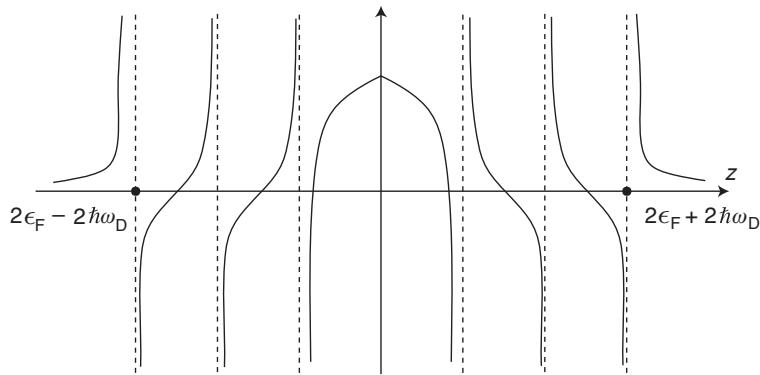
\includegraphics[width=0.62\textwidth]{figs/ch12/fig_12.15.jpg}
\caption*{图 12.15\quad 配对振幅方程的右端作为复能量 $z$ 的函数。}\label{fig:auto:12.15}
\end{figure}

这只有在虚部
\begin{equation*}
\int_{-\hbar\omega_{\mathrm D}}^{\hbar\omega_{\mathrm D}}\frac{\tanh\beta\epsilon/2\,\mathrm d\epsilon}{\left(x-2\epsilon\right)^2+y^2}, \tag{12.143}
\end{equation*}
为零时才成立。因为 $\tanh(x)=-\tanh(-x)$，我们把被积函数改写为
\begin{align*}
0&=\frac{1}{2}\int_{-\hbar\omega_{\mathrm D}}^{\hbar\omega_{\mathrm D}}\mathrm d\epsilon\,\tanh\frac{\beta\epsilon}{2}\left[\frac{1}{\left(x-2\epsilon\right)^2+y^2}-\frac{1}{\left(x+2\epsilon\right)^2+y^2}\right]\\
&=\frac{1}{2}\int_{-\hbar\omega_{\mathrm D}}^{\hbar\omega_{\mathrm D}}\mathrm d\epsilon\,\tanh\frac{\beta\epsilon}{2}\left[\frac{8\epsilon x}{\left(\left(x-2\epsilon\right)^2+y^2\right)\left(\left(x+2\epsilon\right)^2+y^2\right)}\right]. \tag{12.144}
\end{align*}
现在清楚 $x=0$，因为 $\epsilon\tanh\beta\epsilon/2$ 处处为正。因此，我们的解必须形如 $z=2\mu+\mathrm i y$。于是我们必须求解
\begin{equation*}
1=-N\left(\epsilon_{\mathrm F}\right)V_0\int_{-\hbar\omega_{\mathrm D}}^{\hbar\omega_{\mathrm D}}\mathrm d\epsilon\,\frac{\left(-\mathrm i y-2\epsilon\right)\tanh\beta\epsilon/2}{4\epsilon^2+y^2}. \tag{12.145}
\end{equation*}
该积分的虚部关于 $\epsilon$ 为奇，从而严格为零。我们剩下单独一个方程
\begin{equation*}
1=4N\left(\epsilon_{\mathrm F}\right)V_0\int_0^{\hbar\omega_{\mathrm D}}\mathrm d\epsilon\,\frac{\epsilon\tanh\beta\epsilon/2}{4\epsilon^2+y^2}. \tag{12.146}
\end{equation*}
这里被积函数同样是正的。随着 $y$ 增大，被积函数减小。$T$ 增大时也是如此。因此，当 $T$ 大于某个温度时不存在解。这就定义了临界温度 $T_{\mathrm c}$。当 $T\to 0$，我们发现
\begin{align*}
1&=\frac{N\left(\epsilon_{\mathrm F}\right)V_0}{2}\int_0^{(2\hbar\omega_{\mathrm D})^2}\frac{\mathrm d a}{a+y^2}\\
&=\frac{N\left(\epsilon_{\mathrm F}\right)V_0}{2}\ln\left(\frac{(2\hbar\omega_{\mathrm D})^2+y^2}{y^2}\right). \tag{12.147}
\end{align*}
对该方程的两边取指数，
\begin{align*}
y^2&=\left(2\hbar\omega_{\mathrm D}\right)^2\left(\exp\left(\frac{2}{N\left(\epsilon_{\mathrm F}\right)V_0}\right)-1\right)^{-1}\\
&\approx\left(2\hbar\omega_{\mathrm D}\right)^2\exp\left(-\frac{2}{N\left(\epsilon_{\mathrm F}\right)V_0}\right), \tag{12.148}
\end{align*}
得到 $y$ 的熟悉方程，即
\begin{equation*}
y=\pm 2\hbar\omega_{\mathrm D}\exp\left(-\frac{1}{N\left(\epsilon_{\mathrm F}\right)V_0}\right). \tag{12.149}
\end{equation*}
选取正解，我们得出结论：当 $T\to 0$ 时，配对振幅按下式增长：
\begin{align*}
\alpha_{\mathbf p}(t)&\simeq\mathrm e^{-\mathrm i zt}\\
&=\mathrm e^{-2\mathrm i\mu t}\,\mathrm e^{2\hbar\omega_{\mathrm D}t\exp(-1/N(\epsilon_{\mathrm F})V_0)}. \tag{12.150}
\end{align*}
配对振幅指数增长的存在是 $N$ 粒子基态失稳的标志。我们仅仅聚焦于配对振幅 $\alpha_{\mathbf p}$ 就基本上导出了 BCS 理论。为得到 $T_{\mathrm c}$ 的精确表达式，我们在 $y=0$ 的极限下考虑配对结合方程。在此极限下，满足式 (12.146) 的温度最大。因此，$y=0$ 的解可以用来估计 $T_{\mathrm c}$。让我们定义 $\beta_{\mathrm c}=1/k_{\mathrm B}T_{\mathrm c}$。我们发现
\begin{equation*}
1=N\left(\epsilon_{\mathrm F}\right)V_0\int_0^{\hbar\omega_{\mathrm D}\beta_{\mathrm c}/2}\frac{\tanh x}{x}\,\mathrm d x. \tag{12.151}
\end{equation*}
这个积分必须数值完成。与式 (12.151) 一致的转变温度为
\begin{equation*}
k_{\mathrm B}T_{\mathrm c}=1.14\,\hbar\omega_{\mathrm D}\exp\left(-\frac{1}{N\left(\epsilon_{\mathrm F}\right)V_0}\right). \tag{12.152}
\end{equation*}
我们将证明，参数 $y$ 在 BCS 理论中扮演能隙的角色。

\section{BCS 基态}

迄今我们已经展示了配对假设如何在 $T<T_{\mathrm c}$ 时导致基态失稳。现在的焦点是描述这个态的多粒子波函数。我们分析的出发点是 $N$ 个无相互作用电子的多体态：
\begin{equation*}
|\Psi^0(N)\rangle=\prod_{\mathbf p<\mathbf p_{\mathrm F}}b^\dagger_{\mathbf p}|0\rangle. \tag{12.153}
\end{equation*}
由于每个动量态都被双重占据，我们可以用配对算符 $b^\dagger_{\mathbf p}$ 逐次作用于真空来构造这个态。放开 $\mathbf p<\mathbf p_{\mathrm F}$ 的限制，我们把 $|\Psi^0(N)\rangle$ 改写为
\begin{equation*}
\left|\Psi^0\left(N\right)\right.\rangle=\prod_{\mathbf p}\left(u^0_{\mathbf p}+v^0_{\mathbf p}b^\dagger_{\mathbf p}\right)\left|0\right.\rangle, \tag{12.154}
\end{equation*}
其中
\begin{equation*}
u^0_{\mathbf p}=\begin{cases}0, & \mathbf p<\mathbf p_{\mathrm F},\\ 1, & \mathbf p>\mathbf p_{\mathrm F},\end{cases} \tag{12.155}
\end{equation*}
\begin{equation*}
v^0_{\mathbf p}=\begin{cases}1, & \mathbf p<\mathbf p_{\mathrm F},\\ 0, & \mathbf p>\mathbf p_{\mathrm F}.\end{cases} \tag{12.156}
\end{equation*}
$|\Psi^0\rangle$ 的这个表示与式 (12.153) 相同。还要注意，由于诸 $a^\dagger_{\mathbf p}$ 彼此反对易，$|\Psi^0(N)\rangle$ 是恰当反对称化的。

BCS 假定一般的电子超导基态可以写成
\begin{equation*}
|\Psi_{\mathrm{BCS}}\rangle=\prod_{\mathbf p}\left(u_{\mathbf p}+v_{\mathbf p}b^\dagger_{\mathbf p}\right)|0\rangle, \tag{12.157}
\end{equation*}
其中系数 $u_{\mathbf p}$ 与 $v_{\mathbf p}$ 待变分确定，被称为相干因子（coherence factors）。归一化条件 $\langle\Psi_{\mathrm{BCS}}|\Psi_{\mathrm{BCS}}\rangle=1$ 施加约束
\begin{equation*}
1=\langle 0|\prod_{\mathbf p,\mathbf p'}\left(u^*_{\mathbf p}+v^*_{\mathbf p}b_{\mathbf p}\right)\left(u_{\mathbf p'}+v_{\mathbf p'}b^\dagger_{\mathbf p'}\right)|0\rangle. \tag{12.158}
\end{equation*}
式 (12.158) 中出现的这类乘积可以利用式 (12.130) 的对易关系并注意 $b_{\mathbf p}b^\dagger_{\mathbf p}|0\rangle=1$ 来简化。我们发现只有对角 $\left(p=p'\right)$ 项存活：
\begin{equation*}
\langle\Psi_{\mathrm{BCS}}|\Psi_{\mathrm{BCS}}\rangle=\prod_{\mathbf p}\left(\left|u_{\mathbf p}\right|^2+\left|v_{\mathbf p}\right|^2\right), \tag{12.159}
\end{equation*}
这意味着
\begin{equation*}
\left|u_{\mathbf p}\right|^2+\left|v_{\mathbf p}\right|^2=1. \tag{12.160}
\end{equation*}
如果把 BCS 基态中的乘积展开，显然 $|\Psi_{\mathrm{BCS}}\rangle$ 是所有 $2m$ 粒子态的和
\begin{equation*}
|\Psi_{\mathrm{BCS}}\rangle=\sum_m A_{2m}|\Psi_{2m}\rangle, \tag{12.161}
\end{equation*}
其中 $m$ 为整数，$A_{2m}$ 是展开系数，$|\Psi_{2m}\rangle$ 是 $2m$ 个粒子的基态。我们可以通过把展开系数 [S1964] 写成 $A_{2m}=|A_{2m}|\mathrm e^{2\mathrm i m\phi}$ 来建立 $|\Psi_{2m}\rangle$ 与 $|\Psi_{\mathrm{BCS}}\rangle$ 的联系，于是
\begin{equation*}
\left|\Psi^{\phi}_{\mathrm{BCS}}\right.\rangle=\sum_m\mathrm e^{2\mathrm i m\phi}|A_{2m}||\Psi_{2m}\rangle. \tag{12.162}
\end{equation*}
也就是说，我们赋予每个 $2m$ 粒子态一个整体相位 $2m\phi$。为此，通过给每个对产生算符乘上 $\exp(2\mathrm i\phi)$，我们把 BCS 基态改写为
\begin{equation*}
\left|\Psi^{\phi}_{\mathrm{BCS}}\right.\rangle=\prod_{\mathbf p}\left(u_{\mathbf p}+\mathrm e^{2\mathrm i\phi}v_{\mathbf p}b^\dagger_{\mathbf p}\right)\left|0\right.\rangle \tag{12.163}
\end{equation*}
把式 (12.162) 乘以 $\exp(-\mathrm i 2m\phi)$ 并对 $\phi$ 积分，我们得到每个 $2m$ 粒子态与 BCS 基态之间的简洁关系
\begin{equation*}
\left|\Psi_{2m}\right.\rangle=\frac{1}{2\pi\left|A_{2m}\right|}\int_0^{2\pi}\mathrm d\phi\,\mathrm e^{-\mathrm i 2m\phi}\prod_{\mathbf p}\left(u_{\mathbf p}+\mathrm e^{2\mathrm i\phi}v_{\mathbf p}b^\dagger_{\mathbf p}\right)\left|0\right.\rangle \tag{12.164}
\end{equation*}
在式 (12.164) 的右端只有 $2m$ 粒子的态存活，这源于如下事实：
\begin{equation*}
\frac{1}{2\pi}\int_0^{2\pi}\mathrm e^{\mathrm i\phi(N-N')}\mathrm d\phi=\delta_{NN'}. \tag{12.165}
\end{equation*}
由于诸 $2m$ 粒子态相互正交，当我们用 $\langle\Psi_{2m}|$ 乘式 (12.164) 时，左边变为 1，从而可以识别出展开系数的平方为
\begin{align*}
|A_{2m}|^2&=\int_0^{2\pi}\int_0^{2\pi}\frac{\mathrm d\phi}{2\pi}\frac{\mathrm d\phi'}{2\pi}\,\mathrm e^{-\mathrm i 2m(\phi-\phi')}\langle 0|\prod_{\mathbf p,\mathbf p'}\left(u^*_{\mathbf p}+\mathrm e^{-2\mathrm i\phi'}v^*_{\mathbf p}b_{\mathbf p}\right)\left(u_{\mathbf p'}+\mathrm e^{2\mathrm i\phi}v_{\mathbf p'}b^\dagger_{\mathbf p'}\right)|0\rangle\\
&=\frac{1}{2\pi}\int_0^{2\pi}\mathrm d\phi\,\mathrm e^{-2\mathrm i m\phi}\prod_{\mathbf p}\left(\left|u_{\mathbf p}\right|^2+\mathrm e^{2\mathrm i\phi}\left|v_{\mathbf p}\right|^2\right). \tag{12.166}
\end{align*}
式 (12.166) 应被理解为 BCS 态中 $2m$ 个粒子的概率分布。这个量在 BCS 态的平均粒子数处强烈峰化，其宽度正比于系统中平均粒子数的平方根（见习题 12.8）。

我们把 BCS 态改写为所有可能的 $2m$ 粒子态（都具有同一相位 $\phi$）的线性叠加，这暗示在超导态中相位与粒子数之间存在共轭关系。确实存在这样的关系。然而，若其中一个变量有下界，这样的关系便不可能存在。不失一般性，我们可以把粒子数当作 $-\infty<N<\infty$ 的连续变量来处理。我们可以直截了当地建立这一共轭关系：对式 (12.164) 中的 $\left|\psi^{\phi}_{\mathrm{BCS}}\right.\rangle$ 作用 $-\mathrm i\partial/\partial\phi$，然后分部积分。结果
\begin{equation*}
\frac{1}{2\pi|A_{2m}|}\int_0^{2\pi}\mathrm d\phi\,\mathrm e^{-\mathrm i 2m\phi}\frac{-\mathrm i\partial}{\partial\phi}\prod_{\mathbf p}\left(u_{\mathbf p}+\mathrm e^{2\mathrm i\phi}v_{\mathbf p}b^\dagger_{\mathbf p}\right)|0\rangle=2m|\Psi_{2m}\rangle \tag{12.167}
\end{equation*}
暗示粒子数与相位通过
\begin{equation*}
N\leftrightarrow-\mathrm i\frac{\partial}{\partial\phi}, \tag{12.168}
\end{equation*}
相联系，只要我们把粒子数视为连续变量。类似地，把 $\mathrm i\partial/\partial(2m)$ 作用于式 (12.162)，我们类似地确立
\begin{equation*}
\mathrm i\frac{\partial}{\partial N}\leftrightarrow\phi. \tag{12.169}
\end{equation*}
因此，只要把粒子数当作连续变量，相位与粒子数就是共轭的动力学变量。这样，粒子与相位必须满足两个正则共轭变量的海森堡不确定关系 $\Delta\phi\Delta N\ge 2\pi$。于是，相位的完全确定意味着粒子数的无穷不确定，超导体中正是如此。此外，相位与粒子数算符还应满足两个正则共轭变量的哈密顿方程
\begin{align*}
\mathrm i\hbar\dot{\hat N}&=\left[\hat H,\hat N\right]=\mathrm i\frac{\partial\hat H}{\partial\hat\phi},\\
\mathrm i\hbar\dot{\hat\phi}&=\left[\hat H,\hat\phi\right]=-\mathrm i\frac{\partial\hat H}{\partial\hat N} \tag{12.170}
\end{align*}
我们将在本章最后一节表述约瑟夫森效应时使用这些方程。

\section{对涨落}

现在我们来计算 BCS 波函数的 $\langle b_{\mathbf p}\rangle$。在 BCS 基态中，对算符的平均
\begin{align*}
\langle b_{\mathbf p}\rangle_{\mathrm{BCS}}&=\langle 0|\prod_{\mathbf p',\mathbf p''}\left(u^*_{\mathbf p'}+v^*_{\mathbf p'}b_{\mathbf p'}\right)b_{\mathbf p}\left(u_{\mathbf p''}+v_{\mathbf p''}b^\dagger_{\mathbf p''}\right)|0\rangle\\
&=\langle 0|u^*_{\mathbf p}v_{\mathbf p}b_{\mathbf p}b^\dagger_{\mathbf p}|0\rangle=u^*_{\mathbf p}v_{\mathbf p} \tag{12.171}
\end{align*}
不为零。然而在正常态，$u_{\mathbf p}$ 与 $v_{\mathbf p}$ 从不同时非零（见式 (12.155) 与 (12.156)）。因此在正常态 $\langle b_{\mathbf p}\rangle=0$。虽然 $\langle b_{\mathbf p}\rangle$ 在形式上与前几节研究的配对振幅并不相同，但它包含同样的信息。之所以如此，是因为 BCS 基态由具有不同电子数的态组成。某个特定基态的 $\langle b_{\mathbf p}\rangle$ 非零表明该态偏好配对。

于是，合理地定义
\begin{equation*}
\chi=\frac{1}{V}\sum_{\mathbf p}b_{\mathbf p} \tag{12.172}
\end{equation*}
为超导电性的有效序参量。$\chi$ 的平均值
\begin{equation*}
\langle\chi\rangle_{\mathrm{BCS}}=\frac{1}{V}\sum_{\mathbf p}u^*_{\mathbf p}v_{\mathbf p}, \tag{12.173}
\end{equation*}
在超导态有确定的值。为证明这一点，只需证明序参量的二阶涨落为零。我们来计算二阶矩
\begin{equation*}
\langle\chi^2\rangle_{\mathrm{BCS}}=\frac{1}{V^2}\left\langle\sum_{\mathbf p,\mathbf p'}b_{\mathbf p}b_{\mathbf p'}\right\rangle. \tag{12.174}
\end{equation*}
插入 $|\Psi_{\mathrm{BCS}}\rangle$ 后，只有那些动量与式 (12.174) 中指标重合的态才给出非零项。因此，$\langle\chi^2\rangle_{\mathrm{BCS}}$ 是
\begin{equation*}
\frac{1}{V^2}\langle 0|\sum_{\mathbf p,\mathbf p',\mathbf p\neq\mathbf p'}\left(u^*_{\mathbf p}+v^*_{\mathbf p}b_{\mathbf p}\right)\left(u^*_{\mathbf p'}+v^*_{\mathbf p'}b_{\mathbf p'}\right)b_{\mathbf p}b_{\mathbf p'}\left(u_{\mathbf p}+v_{\mathbf p}b^\dagger_{\mathbf p}\right)\left(u_{\mathbf p'}+v_{\mathbf p'}b^\dagger_{\mathbf p'}\right)|0\rangle \tag{12.175}
\end{equation*}
（当 $\mathbf p\neq\mathbf p'$ 时）与
\begin{equation*}
\frac{1}{V^2}\langle 0|\sum_{\mathbf p}\left(u^*_{\mathbf p}+v^*_{\mathbf p}b_{\mathbf p}\right)b^2_{\mathbf p}\left(u_{\mathbf p}+v_{\mathbf p}b^\dagger_{\mathbf p}\right)|0\rangle \tag{12.176}
\end{equation*}
（当 $\mathbf p=\mathbf p'$ 时）之和。第二个表达式因 $\langle b^2_{\mathbf p}\rangle=0$ 而消失。于是 $\langle\chi^2\rangle_{\mathrm{BCS}}$ 在动量空间是非对角的，式 (12.175) 约化为
\begin{align*}
\langle\chi^2\rangle_{\mathrm{BCS}}&=\frac{1}{V^2}\sum_{\mathbf p,\mathbf p',\mathbf p\neq\mathbf p'}u^*_{\mathbf p}v_{\mathbf p}u^*_{\mathbf p'}v_{\mathbf p'}\\
&=\frac{1}{V^2}\sum_{\mathbf p,\mathbf p'}\langle b_{\mathbf p}\rangle\langle b_{\mathbf p'}\rangle\left(1-\delta_{\mathbf p\mathbf p'}\right)\\
&=\langle\chi\rangle^2_{\mathrm{BCS}}-\frac{1}{V^2}\sum_{\mathbf p}\langle b_{\mathbf p}\rangle^2. \tag{12.177}
\end{align*}
序参量的二阶涨落为
\begin{equation*}
\langle\delta\chi^2\rangle=\langle\chi^2\rangle_{\mathrm{BCS}}-\langle\chi\rangle^2_{\mathrm{BCS}}=-\frac{1}{V}\left[\frac{1}{V}\sum_{\mathbf p}\langle b_{\mathbf p}\rangle^2\right]. \tag{12.178}
\end{equation*}
一旦确定了系数 $u_{\mathbf p}$ 与 $v_{\mathbf p}$，我们就能证明 $\langle\delta\chi^2\rangle\propto V^{-1}$，从而在热力学极限下为零。在此基础上，我们将论证 $\langle\chi\rangle$ 在超导态取确定值，并且如前所述，它就是超导转变的序参量。

\section{基态能量}

我们通过在归一化约束（式 (12.160)）与基态能量的粒子数约束下极小化基态能量，来确定系数 $u_{\mathbf p}$ 与 $v_{\mathbf p}$。通过在哈密顿量的平均值中引入一个拉格朗日乘子，我们强制 BCS 基态中的平均粒子数取所需之值（假定为偶数）：
\begin{equation*}
E'=\langle H\rangle-\mu\langle N\rangle, \tag{12.179}
\end{equation*}
其中 $\mu$ 是化学势。为简化计算，我们把单粒子能量重新标度为 $\epsilon_{\mathbf p}\equiv\mathbf p^2/2m-\mu$。于是能量 $E'$ 为
\begin{equation*}
E'=\sum_{\mathbf p,\sigma}\epsilon_{\mathbf p}\langle n_{\mathbf p\sigma}\rangle+\sum_{\mathbf p,\mathbf p'}V_{\mathbf p\mathbf p'}\langle b^\dagger_{\mathbf p}b_{\mathbf p'}\rangle. \tag{12.180}
\end{equation*}
让我们先计算 $\langle n_{\mathbf p\sigma}\rangle$：
\begin{align*}
\langle n_{\mathbf p\sigma}\rangle&=\langle 0|\prod_{\mathbf p'\mathbf p''}\left(u^*_{\mathbf p'}+v^*_{\mathbf p'}b_{\mathbf p'}\right)a^\dagger_{\mathbf p\sigma}a_{\mathbf p\sigma}\left(u_{\mathbf p''}+v_{\mathbf p''}b^\dagger_{\mathbf p''}\right)|0\rangle\\
&=\prod_{\mathbf p',\mathbf p''}\left|v_{\mathbf p'}\right|^2\langle 0|b_{\mathbf p'}n_{\mathbf p\sigma}b^\dagger_{\mathbf p''}|0\rangle\left(\delta_{\mathbf p,\mathbf p'}\delta_{\sigma,\uparrow}+\delta_{\mathbf p,-\mathbf p'}\delta_{\sigma,\downarrow}\right)\\
&=\begin{cases}\left|v_{\mathbf p}\right|^2, & \sigma=\uparrow,\\ \left|v_{-\mathbf p}\right|^2, & \sigma=\downarrow.\end{cases} \tag{12.181}
\end{align*}
反射对称性要求展开系数在 $\mathbf p\to-\mathbf p$ 下不变。$\langle b^\dagger_{\mathbf p}b_{\mathbf p'}\rangle$ 的主导项来自 $\mathbf p\neq\mathbf p'$，因为 $\langle b^2_{\mathbf p}\rangle=0$。此时平均值可以因子化：$\langle b^\dagger_{\mathbf p}b_{\mathbf p'}\rangle=\langle b^\dagger_{\mathbf p}\rangle\langle b_{\mathbf p'}\rangle=u_{\mathbf p}u^*_{\mathbf p'}v^*_{\mathbf p}v_{\mathbf p'}$。于是，基态能量的平均值为
\begin{equation*}
E'=2\sum_{\mathbf p}\left|v_{\mathbf p}\right|^2\epsilon_{\mathbf p}+\sum_{\mathbf p,\mathbf p'}V_{\mathbf p\mathbf p'}u_{\mathbf p}u^*_{\mathbf p'}v^*_{\mathbf p}v_{\mathbf p'}. \tag{12.182}
\end{equation*}
我们需要对 $v^*_{\mathbf p}$ 与 $u^*_{\mathbf p}$ 变分 $E'$
\begin{equation*}
\delta E'=0=2\sum_{\mathbf p}\epsilon_{\mathbf p}\delta v^*_{\mathbf p}v_{\mathbf p}+\sum_{\mathbf p,\mathbf p'}V_{\mathbf p\mathbf p'}\delta v^*_{\mathbf p}\left(u_{\mathbf p}u^*_{\mathbf p'}v_{\mathbf p'}\right)+\sum_{\mathbf p,\mathbf p'}V_{\mathbf p\mathbf p'}\delta u^*_{\mathbf p'}\left(u_{\mathbf p}v^*_{\mathbf p}v_{\mathbf p'}\right), \tag{12.183}
\end{equation*}
以求得最小能量。为消去 $\delta u^*_{\mathbf p'}$，我们注意归一化约束的变分可以改写为
\begin{equation*}
u_{\mathbf p}\delta u^*_{\mathbf p}+v_{\mathbf p}\delta v^*_{\mathbf p}=0 \tag{12.184}
\end{equation*}
或等价地
\begin{equation*}
\delta u^*_{\mathbf p}=-\frac{v_{\mathbf p}}{u_{\mathbf p}}\delta v^*_{\mathbf p}. \tag{12.185}
\end{equation*}
把这个表达式代入式 (12.183) 得到
\begin{equation*}
0=\sum_{\mathbf p}\delta v^*_{\mathbf p}\left[2\epsilon_{\mathbf p}v_{\mathbf p}+\sum_{\mathbf p'}\left[V_{\mathbf p\mathbf p'}\left(u_{\mathbf p}u^*_{\mathbf p'}v_{\mathbf p'}\right)-V_{\mathbf p'\mathbf p}u_{\mathbf p'}v^*_{\mathbf p'}\frac{v^2_{\mathbf p}}{u_{\mathbf p}}\right]\right], \tag{12.186}
\end{equation*}
这意味着
\begin{equation*}
0=2\epsilon_{\mathbf p}v_{\mathbf p}-\Delta_{\mathbf p}u_{\mathbf p}+\Delta^*_{\mathbf p}\frac{v^2_{\mathbf p}}{u_{\mathbf p}}, \tag{12.187}
\end{equation*}
其中我们定义了
\begin{equation*}
\Delta_{\mathbf p}=-\sum_{\mathbf p'}V_{\mathbf p\mathbf p'}u^*_{\mathbf p'}v_{\mathbf p'}. \tag{12.188}
\end{equation*}
我们将看到，$\Delta_{\mathbf p}$ 将扮演能隙的角色。事实上，用 $u_{\mathbf p}$ 去除式 (12.187)，立即可见
\begin{equation*}
0=2\epsilon_{\mathbf p}\frac{v_{\mathbf p}}{u_{\mathbf p}}+\Delta^*_{\mathbf p}\left(\frac{v_{\mathbf p}}{u_{\mathbf p}}\right)^2-\Delta_{\mathbf p}, \tag{12.189}
\end{equation*}
并对这个二次方程解出 $v_{\mathbf p}/u_{\mathbf p}$：
\begin{equation*}
\frac{v_{\mathbf p}}{u_{\mathbf p}}=\frac{-\epsilon_{\mathbf p}\pm\sqrt{\epsilon^2_{\mathbf p}+\left|\Delta_{\mathbf p}\right|^2}}{\Delta^*_{\mathbf p}}. \tag{12.190}
\end{equation*}
让我们定义
\begin{equation*}
\varepsilon_{\mathbf p}\equiv\sqrt{\epsilon^2_{\mathbf p}+\left|\Delta_{\mathbf p}\right|^2}, \tag{12.191}
\end{equation*}
它将被证明是超导态中的准粒子能量。此时我们至少可以启发式地看出，$\Delta_{\mathbf p}$ 确实在单粒子谱 $\epsilon_{\mathbf p}$ 中引入了能隙。注意
\begin{align*}
\frac{v_{\mathbf p}}{u_{\mathbf p}}&=\frac{\epsilon^2_{\mathbf p}-\varepsilon^2_{\mathbf p}}{\left(-\epsilon_{\mathbf p}\mp\varepsilon_{\mathbf p}\right)\Delta^*_{\mathbf p}}\\
&=\frac{\Delta_{\mathbf p}}{\epsilon_{\mathbf p}\pm\varepsilon_{\mathbf p}}, \tag{12.192}
\end{align*}
我们可以把式 (12.190) 进一步简化。在自由系统中当 $\epsilon_{\mathbf p}>\epsilon_{\mathrm F}$ 时 $v_{\mathbf p}/u_{\mathbf p}\to 0$，据此我们判断应当选取 $+$ 号。

结合归一化约束
\begin{equation*}
1=\left|u_{\mathbf p}\right|^2+\left|u_{\mathbf p}\right|^2\frac{\left|\Delta_{\mathbf p}\right|^2}{\left(\epsilon_{\mathbf p}+\varepsilon_{\mathbf p}\right)^2}=2\left|u_{\mathbf p}\right|^2\left[\frac{\varepsilon_{\mathbf p}\left(\epsilon_{\mathbf p}+\varepsilon_{\mathbf p}\right)}{\left(\epsilon_{\mathbf p}+\varepsilon_{\mathbf p}\right)^2}\right], \tag{12.193}
\end{equation*}
我们确定出 $u_{\mathbf p}$ 的大小为
\begin{equation*}
\left|u_{\mathbf p}\right|^2=\frac{\epsilon_{\mathbf p}+\varepsilon_{\mathbf p}}{2\varepsilon_{\mathbf p}}. \tag{12.194}
\end{equation*}
显然，$u_{\mathbf p}$ 的定义带有相位自由度。为简单起见，我们取 $u_{\mathbf p}$ 为正实数。于是我们发现
\begin{equation*}
u_{\mathbf p}=\sqrt{\frac{\epsilon_{\mathbf p}+\varepsilon_{\mathbf p}}{2\varepsilon_{\mathbf p}}} \tag{12.195}
\end{equation*}
以及
\begin{equation*}
v_{\mathbf p}=\frac{\Delta_{\mathbf p}}{\epsilon_{\mathbf p}+\varepsilon_{\mathbf p}}\sqrt{\frac{\epsilon_{\mathbf p}+\varepsilon_{\mathbf p}}{2\varepsilon_{\mathbf p}}}=\sqrt{\frac{\Delta_{\mathbf p}}{\Delta^*_{\mathbf p}}\left(\frac{\varepsilon_{\mathbf p}-\epsilon_{\mathbf p}}{2\varepsilon_{\mathbf p}}\right)}. \tag{12.196}
\end{equation*}
对于所选的简单吸引相互作用，若忽略质心的运动，$\Delta_{\mathbf p}$ 为实数，$v_{\mathbf p}$ 简化为
\begin{equation*}
v_{\mathbf p}=\sqrt{\frac{\varepsilon_{\mathbf p}-\epsilon_{\mathbf p}}{2\varepsilon_{\mathbf p}}}. \tag{12.197}
\end{equation*}
回到确定基态能量的原始问题，我们利用刚导出的相干因子的形式，把平均能量
\begin{align*}
E'_{\mathrm s}&=2\sum_{\mathbf p}\epsilon_{\mathbf p}\left|v_{\mathbf p}\right|^2+\sum_{\mathbf p,\mathbf p'}V_{\mathbf p\mathbf p'}u^*_{\mathbf p'}v_{\mathbf p'}u_{\mathbf p}v^*_{\mathbf p}\\
&=\sum_{\mathbf p}\left(2\epsilon_{\mathbf p}\left|v_{\mathbf p}\right|^2-\Delta_{\mathbf p}u_{\mathbf p}v^*_{\mathbf p}\right)\\
&=-\sum_{\mathbf p}\frac{\left(\varepsilon_{\mathbf p}-\epsilon_{\mathbf p}\right)^2}{2\varepsilon_{\mathbf p}} \tag{12.198}
\end{align*}
约化为单重求和。在没有吸引相互作用时，我们有
\begin{equation*}
E'_n=\sum_{\mathbf p}2\epsilon_{\mathbf p}\theta\left(\mathbf p_{\mathrm F}-\mathbf p\right) \tag{12.199}
\end{equation*}
其中 $\theta$ 是赫维赛德阶跃函数。因为我们已经重新定义 $\epsilon_{\mathbf p}\equiv\mathbf p^2/2m-\mu$，故对 $\mathbf p<\mathbf p_{\mathrm F}$ 有 $\epsilon_{\mathbf p}<0$。于是，超导态与正常态的能量之差由积分
\begin{align*}
\delta E&=-N\left(\epsilon_{\mathrm F}-\mu\right)\left[\int_{-\hbar\omega_{\mathrm D}}^{\hbar\omega_{\mathrm D}}\frac{\left(\varepsilon_{\mathbf p}-\epsilon\right)^2}{2\varepsilon_{\mathbf p}}\,\mathrm d\epsilon+\int_{-\hbar\omega_{\mathrm D}}^{0}2\epsilon\,\mathrm d\epsilon\right]\\
&=-N\left(\epsilon_{\mathrm F}-\mu\right)\int_0^{\hbar\omega_{\mathrm D}}\frac{\left(\varepsilon_{\mathbf p}-\epsilon\right)^2}{\varepsilon_{\mathbf p}}\,\mathrm d\epsilon \tag{12.200}
\end{align*}
给出。为得到最终结果，我们代入 $\varepsilon_{\mathbf p}$ 的表达式并对 $\epsilon$ 积分。在获得最终结果的过程中，引入新变量 $\epsilon=\Delta\sinh y$ 是便利的。于是
\begin{align*}
\left(\varepsilon_{\mathbf p}-\epsilon\right)^2&=\left(\Delta\sqrt{\sinh^2 y+1}-\Delta\sinh y\right)^2\\
&=\left(\Delta\cosh y-\Delta\sinh y\right)^2=\Delta^2\mathrm e^{-2y}. \tag{12.201}
\end{align*}
结果
\begin{equation*}
\delta E=-N\left(\epsilon_{\mathrm F}-\mu\right)\Delta^2\int_0^{\sinh^{-1}(\hbar\omega_{\mathrm D}/\Delta)}\mathrm e^{-2y}\,\mathrm d y. \tag{12.202}
\end{equation*}
一般地，$\hbar\omega_{\mathrm D}/\Delta\gg 1$，因此积分上限可以延拓到 $\infty$。$y$ 积分给出 $1/2$，能量差为
\begin{equation*}
\delta E=\frac{-N\left(\epsilon_{\mathrm F}-\mu\right)\Delta^2}{2}. \tag{12.203}
\end{equation*}
也就是说，超导态的基态能量低于相应正常态的基态能量。超导体中的凝聚能（condensation energy）就是 $\delta E$。

\section{临界磁场}

我们在上一节中证明了超导体中的凝聚能是 $2\delta E=-N\left(\epsilon_{\mathrm F}-\mu\right)\Delta^2$。负号保证超导态能量低于正常态。凝聚能与临界场 $H_{\mathrm c}$ 的关系如下。

考虑把超导体放在如图 12.16 所示的圆柱形几何的磁场中。磁场产生的单位体积能量为 $B^2/8\pi$。

\begin{figure}[H]\centering
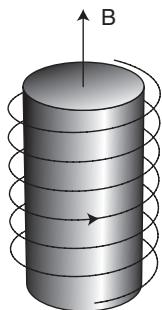
\includegraphics[width=0.34\textwidth]{figs/ch12/fig_12.16.jpg}
\caption*{图 12.16\quad 被磁线圈包围的圆柱形超导体。}\label{fig:auto:12.16}
\end{figure}

磁线圈中的电流由场 $H$ 保持恒定。因此，必然存在矢量场 $\mathbf A(\mathbf r)$ 与磁场产生的电流之间相互作用的贡献。安培定律给出
\begin{equation*}
\nabla\times\mathbf H=\frac{4\pi}{c}\mathbf J, \tag{12.204}
\end{equation*}
其中 $\mathbf J$ 是产生磁场的线圈中的电流。它对能量密度的贡献为
\begin{align*}
W&=-\int\mathbf A\cdot\frac{\nabla\times\mathbf H}{4\pi}\,\frac{\mathrm d\mathbf r}{V}\\
&=-\int\frac{\nabla\times\mathbf A}{4\pi}\cdot\mathbf H\,\frac{\mathrm d\mathbf r}{V}\\
&=-\int\mathbf B\cdot\mathbf H\,\frac{\mathrm d\mathbf r}{4\pi V}. \tag{12.205}
\end{align*}
在均匀系统中 $\mathbf B=\mathbf H$，场导致的总内能为 $H^2/8\pi-H^2/4\pi=-H^2/8\pi$。在正常态，这一能量必须计入总基态能量。因此，存在磁场时正常态的能量为 $E^0_{\mathrm n}=E'_{\mathrm n}-H^2/8\pi$。由于场不穿透超导体，超导体的内能保持 $E'_{\mathrm s}$ 不变。超导电性将持续到 $E'_{\mathrm n}-H^2/8\pi>E'_{\mathrm s}$ 为止。因此
\begin{equation*}
\frac{H^2}{8\pi}>E'_{\mathrm n}-E'_{\mathrm s}=-\delta E \tag{12.206}
\end{equation*}
是场的临界值的判据。我们发现，临界场
\begin{equation*}
H_{\mathrm c}=\sqrt{-8\pi\delta E}=\sqrt{4\pi N\left(\epsilon_{\mathrm F}-\mu\right)}\,\Delta, \tag{12.207}
\end{equation*}
正比于能隙参数 $\Delta$。

\section{能隙}

引入
\begin{align*}
\Delta_{\mathbf p}&=-\sum_{\mathbf p'}V_{\mathbf p\mathbf p'}u^*_{\mathbf p'}v_{\mathbf p'}\\
&=-\sum_{\mathbf p'}V_{\mathbf p\mathbf p'}\frac{\Delta_{\mathbf p'}}{2\varepsilon_{\mathbf p'}}, \tag{12.208}
\end{align*}
作为能隙的物理动机在于：这个量把连续的单粒子谱 $\epsilon_{\mathbf p}$ 劈裂成两支。专门针对只在费米能附近窄动量壳层内非零的模型势，我们把能隙方程改写为
\begin{equation*}
\Delta_{\mathbf p}=V_0{\sum_{\mathbf p'}}\frac{\Delta_{\mathbf p'}}{2\sqrt{\epsilon^2_{\mathbf p'}+\Delta^2_{\mathbf p'}}}. \tag{12.209}
\end{equation*}
求和上的撇号表示限制 $\left|\epsilon_{\mathbf p}-\epsilon_{\mathbf p_{\mathrm F}}\right|<\hbar\omega_{\mathrm D}$。在动量壳层内，只有当费米面各向同性时，$\Delta_{\mathbf p}$ 才相对地与 $\mathbf p$ 无关。对 $s$ 波配对，费米面完全各向同性，能隙可取为与 $\mathbf p$ 无关。对更高角动量的配对态（如 $d$ 波），费米面有节点，能隙的动量依赖不可忽略。为我们的目的，这里我们假定 $\Delta_{\mathbf p}$ 至少在费米面附近的薄动量壳层内与 $\mathbf p$ 无关。能隙方程的一个直接解是 $\Delta=0$。若 $\Delta=0$，则 $\langle b_{\mathbf p}\rangle=0$，从而只可能有正常相。

为得到能隙方程的非平凡解，我们把求和化为积分：
\begin{align*}
1&=N\left(\epsilon_{\mathrm F}-\mu\right)V_0\int_{-\hbar\omega_{\mathrm D}}^{\hbar\omega_{\mathrm D}}\frac{\mathrm d\epsilon}{2\sqrt{\epsilon^2+\Delta^2}}\\
&=N\left(\epsilon_{\mathrm F}-\mu\right)V_0\int_0^{\hbar\omega_{\mathrm D}/\Delta}\frac{\mathrm d\epsilon}{\sqrt{\epsilon^2+1}}\\
&=N\left(\epsilon_{\mathrm F}-\mu\right)V_0\sinh^{-1}\frac{\hbar\omega_{\mathrm D}}{\Delta}. \tag{12.210}
\end{align*}
因此，能隙由下式给出
\begin{equation*}
\Delta=\frac{\hbar\omega_{\mathrm D}}{\sinh\left(1/N\left(\epsilon_{\mathrm F}-\mu\right)V_0\right)}. \tag{12.211}
\end{equation*}
通常，$N\left(\epsilon_{\mathrm F}-\mu\right)V_0\ll 1$。在这个极限下，能隙取熟悉的形式
\begin{equation*}
\Delta(T=0)\simeq 2\hbar\omega_{\mathrm D}\exp\left(-\frac{1}{N(0)V_0}\right). \tag{12.212}
\end{equation*}
在库珀问题中，我们曾证明一个对的结合能与 $\Delta(T=0)$ 相同，只是 $1/\left(N(0)V_0\right)\to 2/\left(N(0)V_0\right)$。在完整理论中，如前所述，费米能以下粒子的配对也被包括进来。因此，精确的指数是 $2/\left(2N(0)V_0\right)=1/\left(N(0)V_0\right)$。在这个意义上，费米面以下粒子的配对有效地使费米能级处的态密度加倍。把能隙与 $T_{\mathrm c}$（式 (12.152)）比较，我们发现
\begin{equation*}
\frac{2\Delta}{k_{\mathrm B}T_{\mathrm c}}=\frac{4\hbar\omega_{\mathrm D}}{1.14\,\hbar\omega_{\mathrm D}}=3.52, \tag{12.213}
\end{equation*}
这是 BCS 理论中的关键比值。它决定超导体是否处于（相对于声子相互作用的）弱耦合极限。强耦合对应 $2\Delta/k_{\mathrm B}T_{\mathrm c}>3.5$。

为计算有限温度下的能隙，我们把费米分布权重因子 $1-n_{\mathbf p\uparrow}-n_{-\mathbf p\downarrow}$ 包括进来，它计及所有粒子之间的配对。因为 $n_{\mathbf p\uparrow}=n_{-\mathbf p\downarrow}$，我们可以把有限温能隙方程写成
\begin{equation*}
\Delta_{\mathbf p}=-\sum_{\mathbf p'}V_{\mathbf p\mathbf p'}\frac{\left(1-2n_{\mathbf p'}\right)}{2\varepsilon_{\mathbf p'}}\Delta_{\mathbf p'}. \tag{12.214}
\end{equation*}
对各向同性系统和 BCS 模型势，我们得到
\begin{equation*}
1=V_0N(0)\int_{-\hbar\omega_{\mathrm D}}^{\hbar\omega_{\mathrm D}}\frac{\tanh\beta\sqrt{\epsilon^2+\Delta^2}/2}{2\sqrt{\epsilon^2+\Delta^2}}\,\mathrm d\epsilon \tag{12.215}
\end{equation*}
作为激发谱中有限温能隙的定义方程。这个方程必须数值求解。不过，其近似解为 $\Delta(T)=\Delta(T=0)\sqrt{1-T/T_{\mathrm c}}$。这一行为如图 12.17 所示。

\begin{figure}[H]\centering
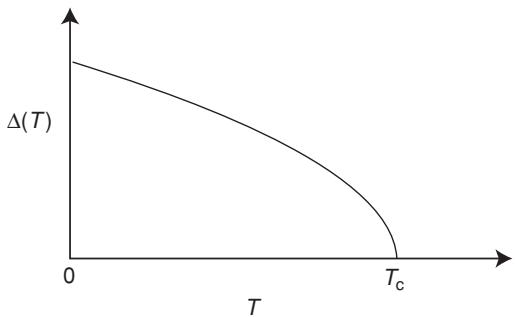
\includegraphics[width=0.5\textwidth]{figs/ch12/fig_12.17.jpg}
\caption*{图 12.17\quad 模型 BCS 相互作用下能隙的渐近行为。渐近地，能隙按 $\Delta(T)=\Delta(T=0)\left(1-\frac{T}{T_{\mathrm c}}\right)^{1/2}$ 标度。}\label{fig:auto:12.17}
\end{figure}

回忆序参量的二阶涨落
\begin{equation*}
\langle\delta\chi^2\rangle=-\frac{1}{V^2}\sum_{\mathbf p}u^{*2}_{\mathbf p}v^2_{\mathbf p}, \tag{12.216}
\end{equation*}
%JOIN%
